\section{Empirical Study Results}
\label{sec:study}
\vspace{-0.2cm}

In this section, we present the details and results of our empirical study. Specifically, we present the study to answer the research questions 1 to 3 in Section~\ref{subsec:pop}, Section~\ref{subsec:usage}, and Section~\ref{subsec:mock}, respectively. We summarize our findings in Section~\ref{subsec:summary}, and present the threats to validity in Section~\ref{subsec:threat}. 
\vspace{-0.2cm}
\subsection{Popularity of Mocking Frameworks}
\label{subsec:pop}
\vspace{-0.2cm}

To answer the first research question, we study the number of software projects using mocking frameworks among the 5,000 downloaded software projects. Specifically, among the 5,000 software projects, 2,046 has at least one test class (a class importing and use any class from JUnit or TestNg). Among the 2,046 projects, 459 projects (23\%) uses at least one mocking framework. We guess that developers of large software projects tend to use mocking frameworks, so we compare the size distribution of software projects using mocking frameworks with the size distribution of all software projects having test code, and present the results in Figure~\ref{fig:box}. The figure shows that the size of software projects using mocking frameworks tends to be larger than other software projects with test code. Specifically, the median size of software projects using mocking frameworks is 16KLOC,  compared to 8.4KLOC of all software projects with test code (software projects in the latter set include software projects in the former set). At the same time, we also found that there are many large software projects do not use any of the investigated mocking frameworks. Furthermore, among the software projects (with test code) that are larger than 10KLOC, and 100KLOC, the proportion of software projects using mocking frameworks goes up to 30\% and 34\%, respectively. 

\begin{figure}
\vspace{-0.3cm}

  \center
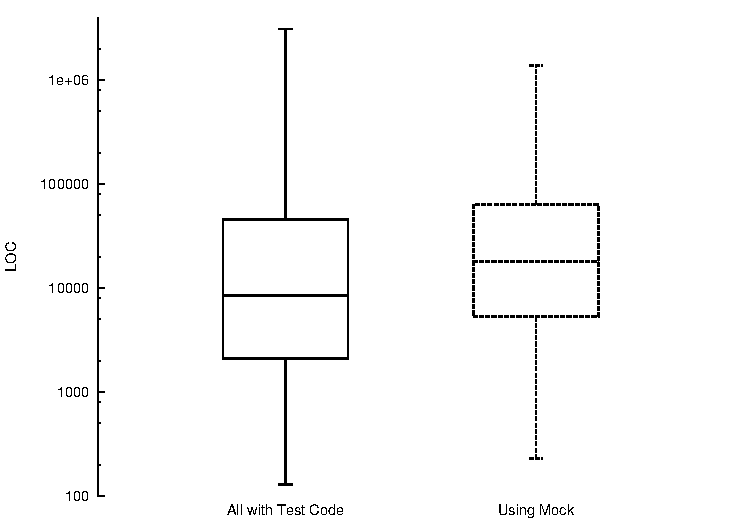
\includegraphics[width=100mm, height=60mm]{boxplot.pdf}
\vspace{-0.3cm}
  \caption{\label{fig:box} Size comparison of software projects using mocking frameworks and all software projects with test code}
  \vspace{-0.3cm}

\end{figure}

                       
On top of the popularity of mocking frameworks in open source software projects, we are also interested in the market share of various popular mocking frameworks. Therefore, we studied the usage of different mocking frameworks and presented the results in Table~\ref{table:var}. From the table, we can see that, among the four major mocking frameworks, Mockito is the most widely used and is used in more than 70\% of software projects that use mocking frameworks. EasyMock and JMock rank second and third, and are used in about 20\% and 10\% of software projects using frameworks, respectively. JMockit is the least widely used among the four. It should be noted that this observation may not be generalized because it is from 5,000 randomly selected Java projects from GitHub. 

Furthermore, we found that 45 software projects use more than one mocking frameworks. We further studied the projects and found that the main reason for software developers to use multiple mocking frameworks is that, different software testers are more familiar with different mocking frameworks so that they use different mocking frameworks in the testing. Another reason is that the software project is moving from one framework to another. 

\begin{table}
\caption{Popularity of Mocking Frameworks}
\vspace{-0.15cm}

\label{table:var}
\centering
\begin{tabular}{|c|r|}
\hline
 Mocking Framework & \# Projects\\
\hline
 Using Mockito & 340\\
 Using EasyMock & 106\\
 Using JMock & 45\\
 Using JMockit & 7\\
 Total & 459\\
 Multiple Mocking Frameworks & 45\\
\hline
\end{tabular}
\vspace{-0.15cm}

\end{table}

We observed that mocking frameworks are used widely in software projects. However, the data above just reveals whether a software project involves mocking frameworks in any test class. It is still not known whether mocking frameworks are used in many test classes or only  a small number of test classes. To answer this question, we further studied the number and proportion of test classes that use mocking frameworks and present the results in Table~\ref{table:testclass}

From the table, we can see that, in software projects that use mocking frameworks, on average, 16.8 test classes are using mocking frameworks, accounting for about 29.8\% of all test classes. This observation shows that software testers are not using mock objects for all dependencies. Also, it is not the case that mock objects are used very rare and in only some special cases. 

\begin{table}
\caption{Usage of Mocking Frameworks in Test Classes}
\vspace{-0.15cm}

\label{table:testclass}
\centering
\begin{tabular}{|c|r|r|r|r|}
\hline
 & Avg. & Med. & Max. & Min\\
\hline
\# Test Files &16.8&5&1037&1\\
Proportion of Test files &29.8\%&20\%&100\%&0.3\%\\
\hline
\end{tabular}
\vspace{-0.15cm}
\end{table}

Moreover, we studied the number of mock objects in one test class and present the results in Table~\ref{table:num}. From the table, we can see that most test classes (77.2\%) have created 3 or less mock objects. Second, we try to understand, for test class that uses mocking frameworks, how many dependency classes are mocked and checked. Specifically, we deem a test class as dependency class if it is imported by the test class. The results are presented in Table~\ref{table:prop}. The table shows that on average about 17\% of dependency classes are mocked by the software testers. Thus, software testers seem to mock only a small portion of all dependency classes of a test class. 

\begin{table}
\caption{Number of Mock Objects in Test Classes}
\vspace{-0.15cm}

\label{table:num}
\centering
\begin{tabular}{|c|r|r|}
\hline
\# Mock Objects & \# Test Files & Proportion\\
\hline
1&1270 & 45.3\%\\
2&587 & 21.0\%\\
3&333 & 11.9\%\\
4&210 & 7.5\%\\
5&135 & 4.8\%\\
6&73 & 2.6\%\\
7&49 & 1.7\%\\
8&40 & 1.4\%\\
9&22 & 0.8\%\\
10+&82 & 2.9\%\\
\hline
\end{tabular}
\vspace{-0.15cm}
\end{table}


\begin{table}
\caption{Proportion of Mocked Classes}
\vspace{-0.15cm}
\label{table:prop}
\centering
\begin{tabular}{|c|r|r|r|r|}
\hline
&Avg. & Med. & Max & Min\\
\hline
\# Mocked Classes &2.7&2&40&1\\
\# Dependency Classes &17.0&14&215&1\\
Proportion of Mocked Clases &17.8\%&14.3\%&100\%&0.9\%\\
\hline
\end{tabular}
\vspace{-0.15cm}
\end{table}

\vspace{-0.2cm}
\subsection{Usage of Mocking Frameworks}
\label{subsec:usage}
\vspace{-0.2cm}

To answer the second research question, we try to study what APIs in mocking frameworks are most widely used. Since different mocking frameworks have different API sets, in this phase, we study only Mockito and EasyMock, which are the most and second most widely used mocking frameworks. The results are presented in Table~\ref{table:mockito} and Table~\ref{table:easymock}

From Table~\ref{table:mockito} and Table~\ref{table:easymock}, we have the following two main observations. First of all, verification of mock objects are extensively used. This fact shows that software testers do not use mocking frameworks simply as a convenient tool for generating normal test stubs or fake objects, but are using the core features of mock objects (i.e., specifying and verifying interactions between the component under test and the software dependency). Second, several advanced APIs in Mockito are widely used. Such APIs include ``spy'' which partially mock an existing class (i.e., use the mock object for specified method invocations, but the real dependency for other method invocations), ``times'' that specify how many times a certain method is invoked, etc. 



\begin{table}
\caption{Most popular ten APIs in Mockito}
\vspace{-0.15cm}
\label{table:mockito}
\centering
\begin{tabular}{|r|r|p{1.3in}|}
\hline
API & Frequency & Description\\
\hline
Mockito.verify&2249 & verify tester's specification of the mock object\\
Mockito.mock&1678 & create an empty mock object\\
Mockito.when&1471 & specify a method in the mock object to be invoked\\
Mockito.spy&403      & partially mock an existing class\\
Mockito.times&232   & specify how many times a method is invoked\\
Mockito.given&161   & Alias of ``when'' for behavior driven development style\\
Mockito.never&152  & specify that a method is never invoked\\
Mockito.verifyNoMoreInteractions & 98 & specify that there are no more interactions between the component under testing and the mock object\\ 
Mockito.doReturn & 85 & specify the return value of a method invocation\\
Mockito.verifyZeroInteractions & 74 & specify that there are no interactions between the component under testing and the mock object\\ 
\hline
\end{tabular}
\vspace{-0.15cm}
\end{table}

\begin{table}
\caption{Most popular ten APIs in EasyMock}
\vspace{-0.15cm}
\label{table:easymock}
\centering
\begin{tabular}{|r|r|p{1.5in}|}
\hline
API & frequency & description\\
\hline
EasyMock.expect&671& specify a method in the mock object to be invoked\\
EasyMock.createmock&647 & create an empty mock object\\
EasyMock.replay&638 & notice the mock object that the testing of component under testing starts\\
EasyMock.verify&510&verify tester's specification of the mock object\\
EasyMock.expectLastCall&144 &alias for ``expect'' for void methods\\
EasyMock.eq & 90 & expect an value that is equals with a given value\\
EasyMock.createNiceMock & 67 &create a mock object that check the order of method invocations\\
EasyMock.anyObject & 64 & match with any type of arguments when specifying the invocation of a method\\
EasyMock.reportMatcher & 58 & specify a matcher of arguments for specification of method invocations\\
EasyMock.capture & 53 & capture a matched value for later access\\
\hline
\end{tabular}
\vspace{-0.15cm}
\end{table}
\vspace{-0.2cm}

\subsection{Mocked Dependencies}
\label{subsec:mock}
\vspace{-0.2cm}

To answer the third research question, we studied the classes that are mocked by software testers using mocking frameworks. Specifically, we try to find out whether software testers tend to mock library classes and what are the mostly mocked library classes. To find the answer, we check whether the mocked classes are library classes (i.e., classes that are not in the source code base of the software project), and present the results in Table~\ref{table:lib}.The results show that about 39\% of all mocked classes are library classes, so software testers actually tend to mock more classes in the source code, compared with library classes. This shows that the major reason for software testers to perform mocking may be parallel development, instead of accelerating testing process and verifying interactions of classes with dependencies. 


\begin{table}
\caption{Mocking of Library Classes}
\vspace{-0.15cm}
\label{table:lib}
\centering
\begin{tabular}{|c|r|r|r|r|}
\hline
&Avg. & Med. & Max & Min\\
\hline
\# Mocked Library Classes &0.85&0.0&18&0\\
Proportion of Library Classes &39.4\%&0\%&100\%&0\%\\
\hline
\end{tabular}
\vspace{-0.15cm}
\end{table}

In Table~\ref{table:mostlib}, we present the top 10 mostly mocked library classes. Specifically, the frequencies are the times that the specific class is mocked in all the studied open source software projects. From the table, we can observe that the two major source of mostly mocked classes are the package ``javax.servlet'', and the package ``javax.jcr''. Specifically, the former package is about HTTP request and responses, and the latter package is about the operation of Java Content Repositories. 

\begin{table}
\caption{Mostly Mocked Library Classes}
\vspace{-0.15cm}
\label{table:mostlib}
\centering
\begin{tabular}{|r|r|}
\hline
Mocked Library Class& Frequency \\
\hline
javax.servlet.http.HttpServletRequest&44\\
org.fest.assertions.description.Description&41\\
javax.servlet.ServletContext&33\\
javax.jcr.Node&32\\
rx.Observer&24\\
org.openqa.selenium.WebDriver&23\\
javax.servlet.http.HttpServletResponse&22\\
javax.jcr.Property&20\\
javax.jcr.Session&20\\
java.io.InputStream&17\\
\hline
\end{tabular}
\vspace{-0.15cm}
\end{table}

\vspace{-0.2cm}
\subsection{Summary}
\label{subsec:summary}
\vspace{-0.2cm}

To sum up, the major findings of our empirical study are as below.
\begin{itemize}
\item Mocking frameworks and mock objects are used widely among open source Java software projects. However, software testers usually mock only a small number and portion of software dependencies.

\item Verification is widely used to check the specified interaction between the component under testing and the mocked object. Special APIs in both Mockito and EasyMock are widely used, which implies an incompleteness of features for a single mocking framework. 

\item Software testers tend to mock source code classes than libraries, while library classes also take a substantial proportion (40\%) in all mocked classes. The mostly mocked library classes are classes from packages handling HTTP requests / responses, and content repositories. 

\end{itemize}
\vspace{-0.3cm}

\subsection{Threats to Validity}
\label{subsec:threat}
\vspace{-0.3cm}

The major threat to the internal validity of our study is the potential errors in the programs analyzing the collected software projects and performing statistics. To reduce the threat, we tried our best to write the code carefully to avoid any bugs in the programs. The major threat to the external validity of our study is that our observations may be specific to the subject software projects, and cannot be generalized other software projects. To reduce this threat, we use a large number of subject software projects, and choose the subjects randomly. Also, it is possible that our findings are specific to Java software projects. To further reduce this threat, we plan to carry out similar empirical studies on subjects written with other major programming languages in the future. 


